% Type of the document
\documentclass{beamer}

% elementary packages:
\usepackage{graphicx}
\usepackage[latin1]{inputenc}
\usepackage[T1]{fontenc}
\usepackage[english]{babel}
\usepackage{listings}
\usepackage{xcolor}
\usepackage{eso-pic}
\usepackage{mathrsfs}
\usepackage{url}
\usepackage{amssymb}
\usepackage{amsmath}
\usepackage{multirow}
\usepackage{hyperref}
\usepackage{booktabs}

% additional packages
\usepackage{bbm}

% packages supplied with ise-beamer:
\usepackage{cooltooltips}
\usepackage{colordef}
\usepackage{beamerdefs}
\usepackage{lvblisting}

% Change the pictures here:
% logobig and logosmall are the internal names for the pictures: do not modify them. 
% Pictures must be supplied as JPEG, PNG or, to be preferred, PDF
\pgfdeclareimage[height=2cm]{logobig}{hulogo}
% Supply the correct logo for your class and change the file name to "logo". The logo will appear in the lower
% right corner:
\pgfdeclareimage[height=0.7cm]{logosmall}{Figures/LOB_Logo}

% Title page outline:
% use this number to modify the scaling of the headline on title page
\renewcommand{\titlescale}{1.0}
% the title page has two columns, the following two values determine the percentage each one should get
\renewcommand{\titlescale}{1.0}
\renewcommand{\leftcol}{0.6}

% Define the title.Don't forget to insert an abbreviation instead 
% of "title for footer". It will appear in the lower left corner:
\title[Prime Numbers and Prime Factorization]{Prime Numbers and Prime Factorization}
% Define the authors:
\authora{Josephine Kraft} % a-c

% Define any internet addresses, if you want to display them on the title page:
\def\linka{http://lvb.wiwi.hu-berlin.de}
\def\linkb{}
\def\linkc{}
% Define the institute:
\institute{Ladislaus von Bortkiewicz Chair of Statistics \\
Humboldt--Universit\"at zu Berlin \\}

% Comment the following command, if you don't want, that the pdf file starts in full screen mode:
\hypersetup{pdfpagemode=FullScreen}

%Start of the document
\begin{document}

% create the title slide, layout controlled in beamerdefs.sty and the foregoing specifications
\frame[plain]{
\titlepage
}

\frame{
\frametitle{Motivation: Cryptography}
\begin{figure}[!t]
\centering

\includegraphics[width=8cm]{cryptography.jpg}
\end{figure}
% Quelle: http://news.sciencemag.org/sites/default/files/styles/thumb_article_l/public/media/sn-cryptography_0.jpg?itok=a4H3ZoHu
}

\frame{
\frametitle{Motivation: Cryptography}

\begin{itemize}
	\item \textbf{Secret key}: two prime numbers p and q
	\item \textbf{Public key}: $p\cdot q$ is used to encrypt messages
	\item Decrypt messages with secret key
	\item Algorithms that find the prime numbers take very long, when only the product is known
	\item Algorithms that find large prime numbers are needed
\end{itemize}

% Quelle: http://www.arndt-bruenner.de/mathe/scripts/primzahlen.htm#probaerkl
}

%%%%%%%%%%%%%%%%%%%%%%%%%%%%%%%%%%%%%%%%%%%%%%%%%%%%%%%%%%%%%%%%%%%%%%%%%%%%%%%%%%%%%%%%%%%%%%%%%%%%%%%%%%%%%%%%%%%%%%%%
\frame{
\frametitle{Outline}

\begin{enumerate}
\item Introduction
\item Prime Factorization
\item Finding Prime Numbers
			\begin{enumerate}
				\item Sieve of Eratosthenes
				\item Sieve of Atkin and Bernstein
			\end{enumerate}
\end{enumerate}
}

%%%%%%%%%%%%%%%%%%%%%%%%%%%%%%%%%%%%%%%%%%%%%%%%%%%%%%%%%%%%%%%%%%%%%%%%%%%%%%%%%%%%%%%%%%%%%%%%%%%%%%%%%%%%%%%%%%%%%%%%
\section{Introduction}
%%%%%%%%%%%%%%%%%%%%%%%%%%%%%%%%%%%%%%%%%%%%%%%%%%%%%%%%%%%%%%%%%%%%%%%%%%%%%%%%%%%%%%%%%%%%%%%%%%%%%%%%%%%%%%%%%%%%%%%%
%\frame{
%\frametitle{Cryptography}

%\begin{itemize}
%\item \texttt{Beamer} is the latest package to create slides with \LaTeX
%\item Slides need to be compiled to PDF, not DVI/Postscript
%\item Remember: PDFLaTeX accepts PNG, JPEG and PDF not EPS/PS
%\item If you \emph{need} Postscript, RTFM
%\end{itemize}

%}

%%%%%%%%%%%%%%%%%%%%%%%%%%%%%%%%%%%%%%%%%%%%%%%%%%%%%%%%%%%%%%%%%%%%%%%%%%%%%%%%%%%%%%%%%%%%%%%%%%%%%%%%%%%%%%%%%%%%%%%%
\frame{
\frametitle{What are Prime Numbers?}

\begin{itemize}
\item A \textbf{prime number} is an integer $p>1$ which has exactly two positive divisors, namely $1$ and $p$
\item An integer n is \textbf{composite} or \textbf{non prime} if and only if it admits a nontrivial factorization $n=ab$, where $a$ and $b$ are integers, $1<a,b<n$
\item The resulting sequence of prime numbers is: 2, 3, 5, 7, 11, 13, 17, 19, 23, 29, 31, 37, 41, 43, 47, 53, 59, ...
\end{itemize}
}

%%%%%%%%%%%%%%%%%%%%%%%%%%%%%%%%%%%%%%%%%%%%%%%%%%%%%%%%%%%%%%%%%%%%%%%%%%%%%%%%%%%%%%%%%%%%%%%%%%%%%%%%%%%%%%%%%%%%%%%%
\section{Prime Factorization}
%%%%%%%%%%%%%%%%%%%%%%%%%%%%%%%%%%%%%%%%%%%%%%%%%%%%%%%%%%%%%%%%%%%%%%%%%%%%%%%%%%%%%%%%%%%%%%%%%%%%%%%%%%%%%%%%%%%%%%%%

\frame{
\frametitle{Prime Factorization}

\begin{theorem}[Fundamental Theorem of Arithmetic]\\
For each natural number n there is a unique factorization
\begin{equation*}
%n=p_1^{a_1} \cdot \ldots \cdot p_k^{a_k}
n=\prod_{i=1}^{k} p_i^{a_i}
\end{equation*}
where all $a_i$ are positive integers and $p_1,...,p_k$ are primes.
\end{theorem}

\textbf{$\to$ Fundamental Problem of Arithmetic}
}

%%%%%%%%%%%%%%%%%%%%%%%%%%%%%%%%%%%%%%%%%%%%%%%%%%%%%%%%%%%%%%%%%%%%%%%%%%%%%%%%%%%%%%%%%%%%%%%%%%%%%%%%%%%%%%%%%%%%%%%%
%\subsection{Distribution of Primes}

%\frame{
%\frametitle{Distribution of Primes}

%\begin{itemize}
%	\item Denote by $\mathcal{P}$ the set of all primes. The \textbf{prime-counting function} at real values $x$  is defined as
%				\begin{equation*}
%					\pi(x)=\#\{p\leq x | p\in\mathcal{P}\}
%				\end{equation*}
%	\item Growth rate: \[\pi(x)\sim \frac{x}{\ln(x)},\ i.e.\ \lim\limits_{x \rightarrow \infty}{\frac{\pi(x)}{\frac{x}{\ln(x)}}} = 1\]
%\end{itemize}

%}

%%%%%%%%%%%%%%%%%%%%%%%%%%%%%%%%%%%%%%%%%%%%%%%%%%%%%%%%%%%%%%%%%%%%%%%%%%%%%%%%%%%%%%%%%%%%%%%%%%%%%%%%%%%%%%%%%%%%%%%%

%\frame{
%\frametitle{Distribution of Primes}

%\begin{figure}[!h]
%\centering
%\includegraphics[width=6.5cm]{prime_counting_function.jpeg}
%%\caption{Prime-counting function}
%\end{figure}
%}

%%%%%%%%%%%%%%%%%%%%%%%%%%%%%%%%%%%%%%%%%%%%%%%%%%%%%%%%%%%%%%%%%%%%%%%%%%%%%%%%%%%%%%%%%%%%%%%%%%%%%%%%%%%%%%%%%%%%%%%%
\section{Sieve of Eratosthenes}
%%%%%%%%%%%%%%%%%%%%%%%%%%%%%%%%%%%%%%%%%%%%%%%%%%%%%%%%%%%%%%%%%%%%%%%%%%%%%%%%%%%%%%%%%%%%%%%%%%%%%%%%%%%%%%%%%%%%%%%%

\frame{
\frametitle{Sieve of Eratosthenes}

% Quelle Bild: https://camo.githubusercontent.com/8c51c16c0ff79a2ca8cfe07b08f9a000ed149308/687474703a2f2f6661726d352e7374617469632e666c69636b722e636f6d2f343132372f353132383336313036305f613136636262353332332e6a7067

\begin{figure}[!h]
\centering
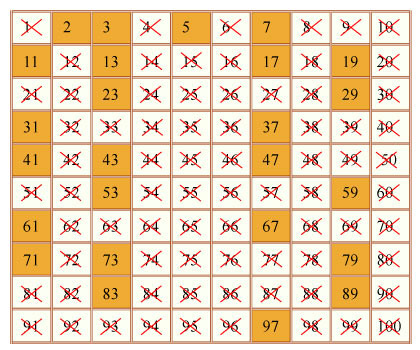
\includegraphics[width=7cm]{sieve_of_eratosthenes.jpg}
\end{figure}
}



%%%%%%%%%%%%%%%%%%%%%%%%%%%%%%%%%%%%%%%%%%%%%%%%%%%%%%%%%%%%%%%%%%%%%%%%%%%%%%%%%%%%%%%%%%%%%%%%%%%%%%%%%%%%%%%%%%%%%%%%

\frame{
\frametitle{Algorithm}

\begin{itemize}
	\item Aim: Find all prime numbers up to $N=30$
	\item Cross from list all multiples of each prime number, starting with the multiples of 2
\end{itemize}

\begin{figure}[!h]
\centering
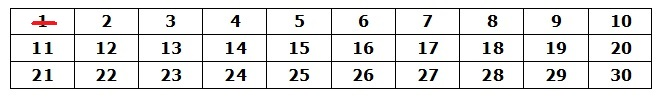
\includegraphics[width=10cm]{example2.jpg}
\end{figure}

\begin{figure}[!h]
\centering
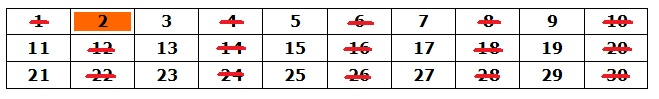
\includegraphics[width=10cm]{example3.jpg}
\end{figure}

}

\frame{
\frametitle{Algorithm}

\begin{figure}[!h]
\centering
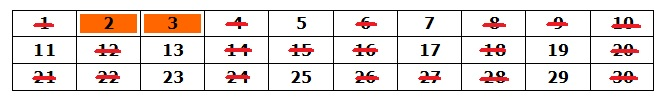
\includegraphics[width=10cm]{example4.jpg}
\end{figure}

\begin{figure}[!h]
\centering
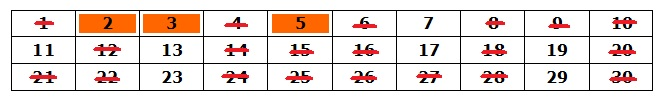
\includegraphics[width=10cm]{example5.jpg}
\end{figure}

\begin{figure}[!h]
\centering
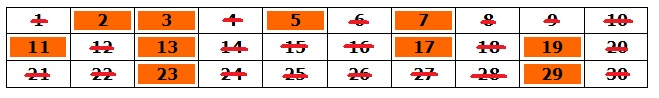
\includegraphics[width=10cm]{example6.jpg}
\end{figure}

}

\frame{
\frametitle{R Code}

\begin{figure}[!h]
\centering
\fbox{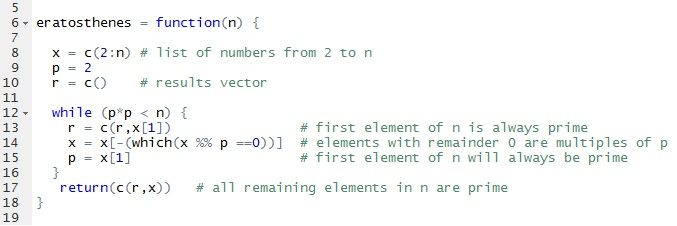
\includegraphics[width=11cm]{code_eratosthenes.jpg}}
\end{figure}

}

\frame{
\frametitle{R Code: Results}

\begin{figure}[!h]
\centering
\fbox{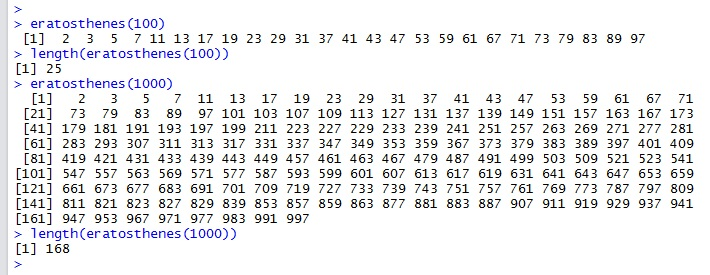
\includegraphics[width=11cm]{results_eratosthenes2.jpg}}
\end{figure}

}

%\frame[containsverbatim]{
%\frametitle{R-Code}
%\begin{lstlisting}
%eratosthenes <- function(n){
%  a = c(2:n) # List of numbers from 2 to n
%  p = 2 # Prime number you look at. Initially p=2
%  r = c() # Results list
%    
%  while (p*p < n) {
%      r = c(r,a[1])
%      a = a[-(which(a %% p ==0))]
%      p = a[1]
%    }
%  c(r,a)
%}
%\end{lstlisting}
%}

%%%%%%%%%%%%%%%%%%%%%%%%%%%%%%%%%%%%%%%%%%%%%%%%%%%%%%%%%%%%%%%%%%%%%%%%%%%%%%%%%%%%%%%%%%%%%%%%%%%%%%%%%%%%%%%%%%%%%%%%%

%\frame{
%\frametitle{Complete Factorizations}

%\begin{figure}[!h]
%\centering
%\includegraphics[width=11cm]{factorization_neu3.jpg}
%\end{figure}

%}

%%%%%%%%%%%%%%%%%%%%%%%%%%%%%%%%%%%%%%%%%%%%%%%%%%%%%%%%%%%%%%%%%%%%%%%%%%%%%%%%%%%%%%%%%%%%%%%%%%%%%%%%%%%%%%%%%%%%%%%%%
\section{Sieve of Atkin and Bernstein}
%%%%%%%%%%%%%%%%%%%%%%%%%%%%%%%%%%%%%%%%%%%%%%%%%%%%%%%%%%%%%%%%%%%%%%%%%%%%%%%%%%%%%%%%%%%%%%%%%%%%%%%%%%%%%%%%%%%%%%%%%

\frame{
\frametitle{Sieve of Atkin and Bernstein}

\begin{itemize}
	\item Introduced in 2003 by Arthur O.L. Atkin and Daniel J. Bernstein
	\item All primes (except 2 and 3) are of one of the following forms:\\
				\begin{itemize}
					\item \textbf{Group 1:} $n\equiv 1\ \ (mod\ 4)\ \iff\ n=4k + 1$ 
					\item	\textbf{Group 2:} $n\equiv 1\ \ (mod\ 6)\ \iff\ n=6k + 1$ 
					\item	\textbf{Group 3:} $n\equiv 11\ \ (mod\ 12)\ \iff\ n=12k + 11$
				\end{itemize}
				with $k\in\mathbb{N}_{0}$
	\item The algorithm is based on three theorems, one theorem for each group of primes
\end{itemize}

}

%%%%%%%%%%%%%%%%%%%%%%%%%%%%%%%%%%%%%%%%%%%%%%%%%%%%%%%%%%%%%%%%%%%%%%%%%%%%%%%%%%%%%%%%%%%%%%%%%%%%%%%%%%%%%%%%%%%%%%%%%%

\frame{
\frametitle{Theory}

\begin{theorem}[1]
Let n be a squarefree positive integer with $n\equiv 1\ \ (mod\ 4)$. Then n is prime if and only if the cardinality of the following set is odd: 
\begin{equation*}
	\{(x,y)\ |\ 4x^2+y^2=n,\ x,y\in\mathbb{N}\}
\end{equation*}
\end{theorem}

\underline{Remark:} \\ A \textbf{squarefree number} is an integer, which is divisible by no other square number than 1. \\ Equivalently, an integer is squarefree if and only if in its prime factorization no prime factor occurs more than once.

%\begin{itemize}
	%\item A \textbf{squarefree number} is an integer, which is divisible by no other square number than 1. Equivalently, an integer is %squarefree if and only if in its prime factorization no prime factor occurs more than once.
%\end{itemize}

}

%%%%%%%%%%%%%%%%%%%%%%%%%%%%%%%%%%%%%%%%%%%%%%%%%%%%%%%%%%%%%%%%%%%%%%%%%%%%%%%%%%%%%%%%%%%%%%%%%%%%%%%%%%%%%%%%%%%%%%%%%%%%%%%%%%%%%

\frame{
\frametitle{Theory}

\begin{theorem}[2]
Let n be a squarefree positive integer with $n\equiv 1\ \ (mod\ 6)$. Then n is prime if and only if the cardinality of the following set is odd: 
\begin{equation*}
	\{(x,y)\ |\ 3x^2+y^2=n,\ x,y\in\mathbb{N}\}
\end{equation*}
\end{theorem}

\begin{theorem}[3]
Let n be a squarefree positive integer with $n\equiv 11\ \ (mod\ 12)$. Then n is prime if and only if the cardinality of the following set is odd: 
\begin{equation*}
	\{(x,y)\ |\ 3x^2-y^2=n,\ x,y\in\mathbb{N}, x>y\}
\end{equation*}
\end{theorem}

}

%\frame{
%\frametitle{Theory}

%\begin{itemize}
%	\item \textbf{1. Group:} $n=4k+1\ \to\ n\in\{1,5,9,13,17,21,...\}$
%		\begin{itemize}
%			\item Equivalently: $n=60k+r$, where $k\in\mathbb{N}_{0}$ and $r\in\{1,5,9,13,17,21,25,29,33,37,41,45,49,53,57\}$
%		\end{itemize}
%	\item \textbf{2. Group:} $n=6k+1\ \to\ n\in\{1,7,13,19,25,31,...\}$
%		\begin{itemize}
%			\item Equivalently: $n=60k+r$, where $k\in\mathbb{N}_{0}$ and $r\in\{1,7,13,19,25,31,37,43,49,55\}$
%		\end{itemize}
%	\item \textbf{3. Group:} $n=12k+11\ \to\ n\in\{11,23,35,47,59,...\}$
%		\begin{itemize}
%			\item Equivalently: $n=60k+r$, where $k\in\mathbb{N}_{0}$ and $r\in\{11,23,35,47,59\}$
%		\end{itemize}
%\end{itemize}  
%}

%\frame{
%\frametitle{Theory}

%\textbf{Remark:} If there exists an integer g such that g divides m and r. Then g also divides $n=m\cdot k\ +\ r$ with $k\in\mathbb{N}_{0}$. This implies that n is not a prime number. \\

%\textbf{Example:} $m=60$ has divisors 2,3 and 5.
%In the 1. group remainders 9, 21, 33, 45, 57 have divisor 3. $\to$ Remove!

%}

\frame{
\frametitle{Theory}

\begin{itemize}
	\item All numbers of the 3 groups can be represented in the form $60k + r$, with varying values for r
	\vspace{3mm}
	\pause
	\item Modified groups to consider in algorithm:
	\pause
		\begin{itemize}
			\item \textbf{1. Group:} $n=60k+r$, where $k\in\mathbb{N}_{0}$ and $r\in\{1,13,17,29,37,41,49,53\}$
			\vspace{3mm}
			\pause
			\item \textbf{2. Group:} $n=60k+r$, where $k\in\mathbb{N}_{0}$ and \\ $r\in\{7,19,31,43\}$
			\vspace{3mm}
			\pause
			\item \textbf{3. Group:} $n=60k+r$, where $k\in\mathbb{N}_{0}$ and \\ $r\in\{11,23,47,59\}$
		\end{itemize}
\end{itemize}

}

\frame{
\frametitle{Theory}
\begin{theorem}[1]
Let n be a squarefree positive integer with $n\equiv 1\ \ (mod\ 4)$. Then n is prime if and only if \#$\{(x,y)\ |\ 4x^2+y^2=n,\ x,y\in\mathbb{N}\}$ is odd.
\end{theorem}

\begin{theorem}[2]
Let n be a squarefree positive integer with $n\equiv 1\ \ (mod\ 6)$. Then n is prime if and only if \#$\{(x,y)\ |\ 3x^2+y^2=n,\ x,y\in\mathbb{N}\}$ is odd.
\end{theorem}

\begin{theorem}[3]
Let n be a squarefree positive integer with $n\equiv 11\ \ (mod\ 12)$. Then n is prime if and only if \#$\{(x,y)\ |\ 3x^2-y^2=n,\ x,y\in\mathbb{N},\ x>y\}$ is odd.
\end{theorem}

}

\frame{
\frametitle{Algorithm}

\begin{enumerate}
	\item Create sieve list with N entries,  where each number is initially marked as non prime.
	\vspace{2mm}
	\pause
	\item For each $n\leq N$: Calculate modulo-60 remainder of n.
	\vspace{2mm}
	\pause
		\begin{itemize}
			\item \textbf{If} $\boldsymbol{r\in\{1,13,17,29,37,41,49,53\}}$: \\ Change $n^{th}$ entry in sieve list from prime to non prime (or vice versa) $\forall$ (x,y) with $4x^2+y^2=n$, $x,y\in\mathbb{N}$.
			\vspace{2mm}
			\pause
			\item \textbf{If} $\boldsymbol{r\in\{7,19,31,43\}}$: \\ Change $n^{th}$ entry in sieve list from prime to non prime (or vice versa) $\forall$ (x,y) with $3x^2+y^2=n$, $x,y\in\mathbb{N}$.
			\vspace{2mm}
			\pause
			\item \textbf{If} $\boldsymbol{r\in\{11,23,47,59\}}$: \\ Change $n^{th}$ entry in sieve list from prime to non prime (or vice versa) $\forall$ (x,y) with $3x^2-y^2=n$, $x,y\in\mathbb{N}$.
		\end{itemize}
\end{enumerate}
}

\frame{
\frametitle{Algorithm}

\begin{enumerate}
	\setcounter{enumi}{2}
	\item There are still non-squarefree integers that could be marked as prime $\to$ Start with lowest number p marked as prime. Change entry for all multiples of the square of p \textit{($p^2,2p^2,3p^2,4p^2,... $)} to non prime. Repeat until $p^2 > N$.
\end{enumerate}
}

\frame{
\frametitle{R Code}

\begin{figure}[!h]
\centering
\fbox{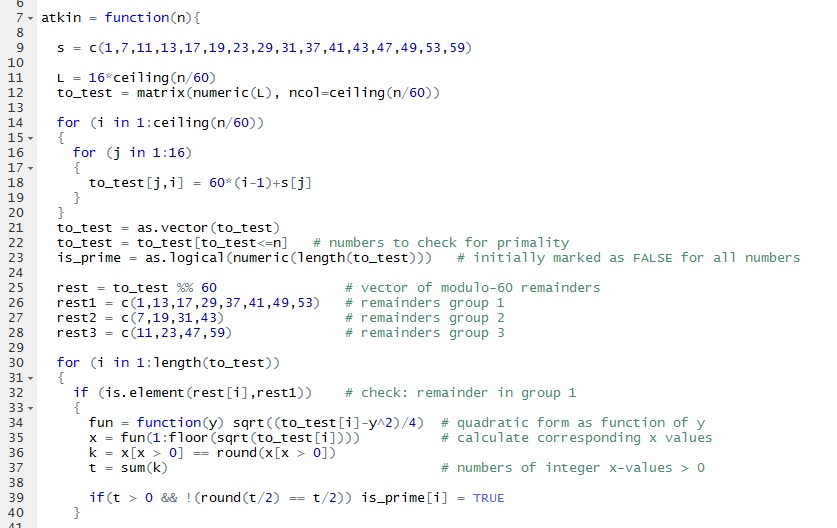
\includegraphics[width=9.5cm]{code_atkin1.jpg}}
\end{figure}

}

\frame{
\frametitle{R Code}

\begin{figure}[!h]
\centering
\fbox{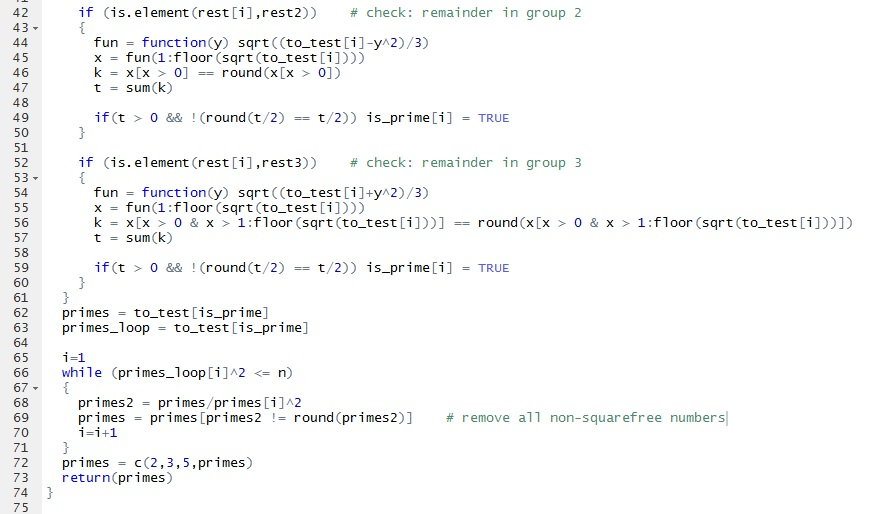
\includegraphics[width=9.5cm]{code_atkin2.jpg}}
\end{figure}

}

\frame{
\frametitle{R Code: Results}

\begin{figure}[!h]
\centering
\fbox{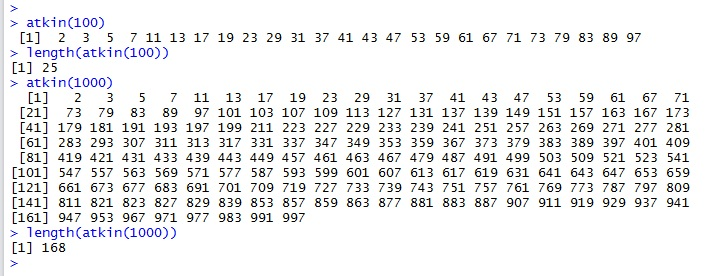
\includegraphics[width=9.5cm]{results_atkin.jpg}}
\end{figure}

}

\section{Sieve of Eratosthenes vs. Sieve of Atkin and Bernstein}

\frame{
\frametitle{Finding Large Prime Numbers}

\begin{tabular}{ccc}
	\hline
	Test for $N=10^8$	& \textbf{Eratosthenes} & \textbf{Atkin \& Bernstein} \\
	\hline \hline
	\textbf{Primes found} &  5,761,455 & 5,761,455 \\
	\textbf{Largest Prime} & 99,999,989 & 99,999,989 \\
	\textbf{Running Time} & 4.5 min & 6.2 hours \\
	\hline
\end{tabular}\\
\vspace{5mm}
\begin{tabular}{cc}
	\hline
	Test for $N=10^9$	& \textbf{Eratosthenes} \\
	\hline \hline
	\textbf{Primes found} &  50,847,534 \\
	\textbf{Largest Prime} & 999,999,937 \\
	\textbf{Running Time} & 1.7 hours \\
	\hline
\end{tabular}

}
%%%%%%%%%%%%%%%%%%%%%%%%%%%%%%%%%%%%%%%%%%%%%%%%%%%%%%%%%%%%%%%%%%%%%%%%%%%%%%%%%%%%%%%%%%%%%%%%%%%%%%%%%%%%%%%%%%%%%%%%%%%%%%%%%%%%%%

\section{}

\frame{
\frametitle{Thank you for your Attention!}

\begin{center}\begin{Large}\textbf{Enter any 11-digit prime number to\\ \vspace{3mm} continue ...}\end{Large}\end{center}

}

%%%%%%%%%%%%%%%%%%%%%
\section{Bibliography}
%%%%%%%%%%%%%%%%%%%%%%%%%%%%%%%%%%%%%%%%%%%%%%%%%%%%%

%%%%%%%%%%%%%%%%%%%%%%%%%%%%%%%%%%%%%%%%%%%%%%%%%%%%%
\frame{
\frametitle{Bibliography}

\begin{thebibliography}{aaaaaaaaaaaaaaaaa}

\beamertemplatearticlebibitems
\bibitem{Atkin:2003}
A. O. L. Atkin, D. J. Bernstein
\newblock{\em Prime Sieves using binary quadratic forms}
\newblock available on \href{http://www.ams.org/journals/mcom/2004-73-246/S0025-5718-03-01501-1/S0025-5718-03-01501-1.pdf}{http://www.ams.org/journals/mcom}, 2003.
      
\beamertemplatebookbibitems
\bibitem{Crandall:2005}
R. Crandall, C. Pomerance
\newblock{\em Prime Numbers. A Computational Perspective}
\newblock Springer 2005. 

\beamertemplatebookbibitems
\bibitem{Joux:2005}
A. Joux
\newblock{\em Algorithmic Cryptanalysis}
\newblock Chapman & Hall/CRC 2009. 

\end{thebibliography}
} %end of frame

% Define the end of the document:
\end{document}
